\documentclass[11pt]{beamer}
\usepackage{tikz}
\usetheme{Warsaw}
% AIMS official logo colour
\definecolor{checkers}{RGB}{96,180,181}
\usecolortheme[named=checkers]{structure}
% packages
\usepackage[utf8]{inputenc}
\usepackage{hyperref}
\usepackage{amsmath}
\usepackage{amsfonts}
\usepackage{amssymb}
\usepackage{graphicx}
\usepackage{caption}
\captionsetup[figure]{labelformat=empty}
\title{Decision Tree Learning}
\author{Reem Elmahdi}
%\setbeamercovered{transparent} 
%\setbeamertemplate{navigation symbols}{} 
%\logo{\includegraphics[scale=0.35]{checkers_logo}} 
\institute{African Institute For Mathematical Sciences
\newline \newline
Interdisciplinary Center for Scientific Computing (IWR)}
%\date{} 
%\subject{} 
\begin{document}

\begin{frame}
\titlepage
\end{frame}

\usebackgroundtemplate{%
\tikz[overlay,remember picture] \node[opacity=0.3, at=(current page.center)] {
   
\includegraphics[height=\paperheight,width=\paperwidth]{0}};
}

\begin{frame}{Who am I?}	

\begin{itemize}
\item \textbf{Reem Omer;} \newline
\item \textbf{Graduated from Sudan University of Science and Technology;}\newline
\item \textbf{Computer and Information Systems;} \newline
\item \textbf{A master student at AIMS;}\newline
\item \textbf{Machine Learning and Big Data.}
\end{itemize}
\end{frame}
%%%%%%%%%%%%%%%%%%%%%%%%%%%%%%%%%%%%%%%%%%%%%%%%%%%%%%%%%%%%%%%%%%%%%%%%%%%%%%%%%%%%
\usebackgroundtemplate{}
\begin{frame}{Machine Learning}

\includegraphics[scale=0.2]{1}
\end{frame}
%%%%%%%%%%%%%%%%%%%%%%%%%%%%%%%%%%%%%%%%%%%%%%%%%%%%%%%%%%%%%%%%%%%%%%%%%%%%%%%%%%%%
\begin{frame}{Example in Machine Learning:}
\textbf{Can you write a code to tell the difference between apples and oranges?}
\begin{center}
\begin{figure}[H]
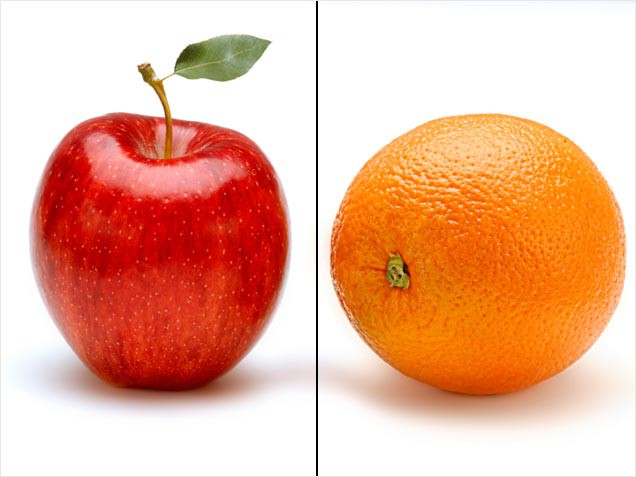
\includegraphics[scale=0.3]{2}
\end{figure}
\end{center}
\end{frame}
%%%%%%%%%%%%%%%%%%%%%%%%%%%%%%%%%%%%%%%%%%%%%%%%%%%%%%%%%%%%%%%%%%%%%%%%%%%%%%%%%%%%
\begin{frame}{Iris Flower Data Set:}
\textbf{We have three types of Iris flower, and our goal is to identify type of flower.}

\begin{figure}[!htb]
\minipage{0.32\textwidth}
  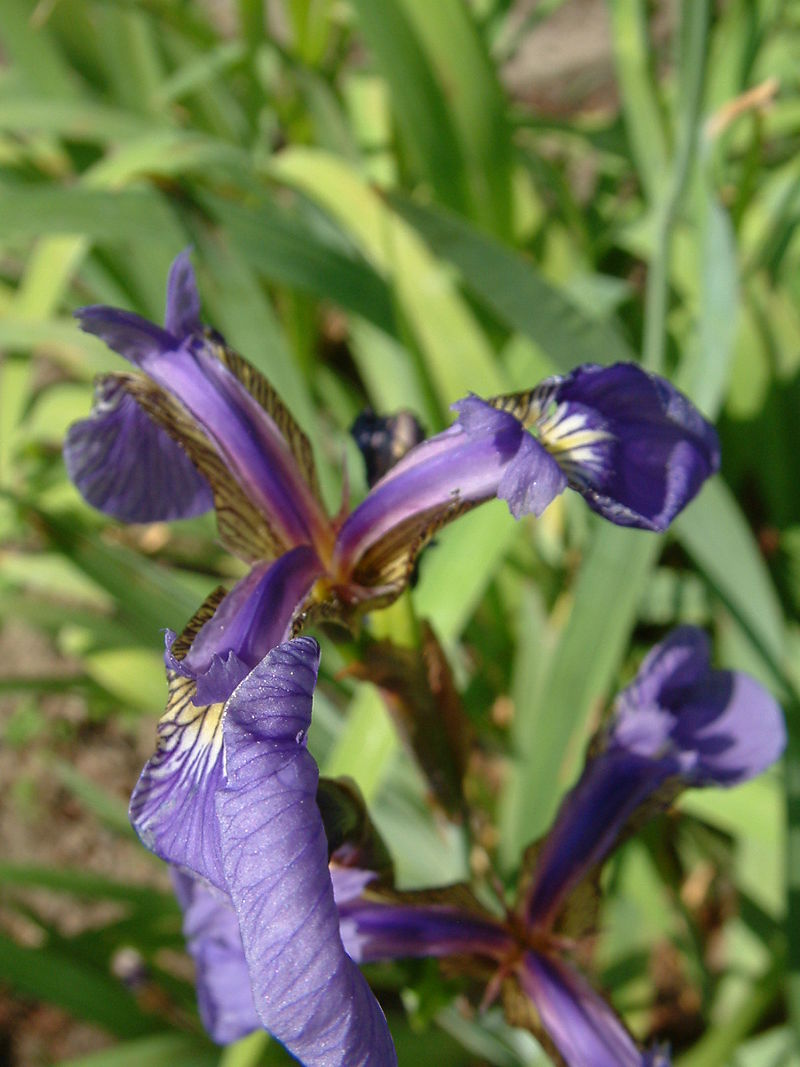
\includegraphics[width=3cm,height=3cm]{setosa}
  \caption{$\textit{Setosa}$}
\endminipage\hfill
\minipage{0.32\textwidth}
  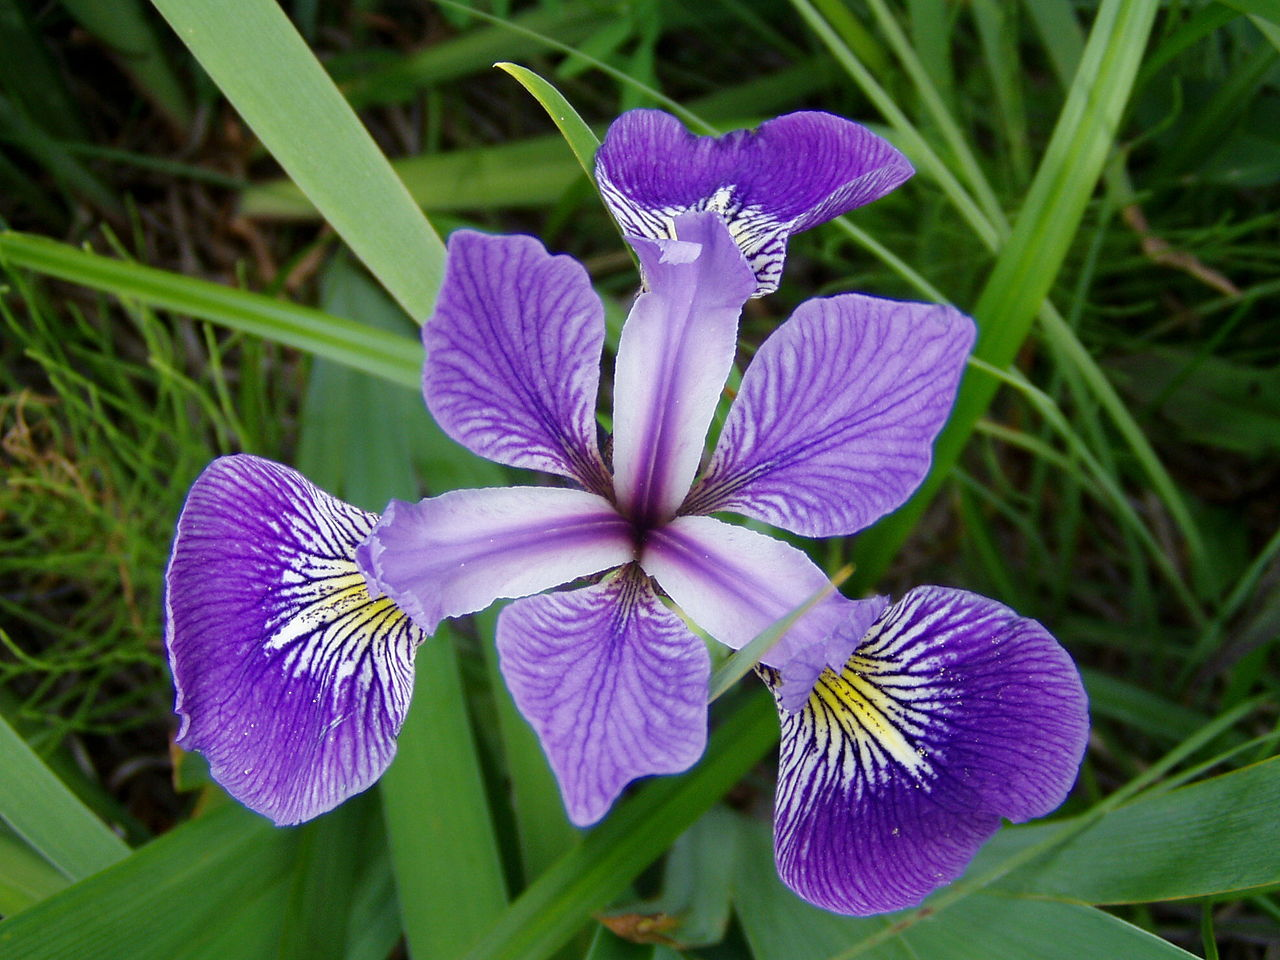
\includegraphics[width=3cm,height=3cm]{versicolor}
  \caption{$\textit{Versicolor}$}
\endminipage\hfill
\minipage{0.32\textwidth}%
  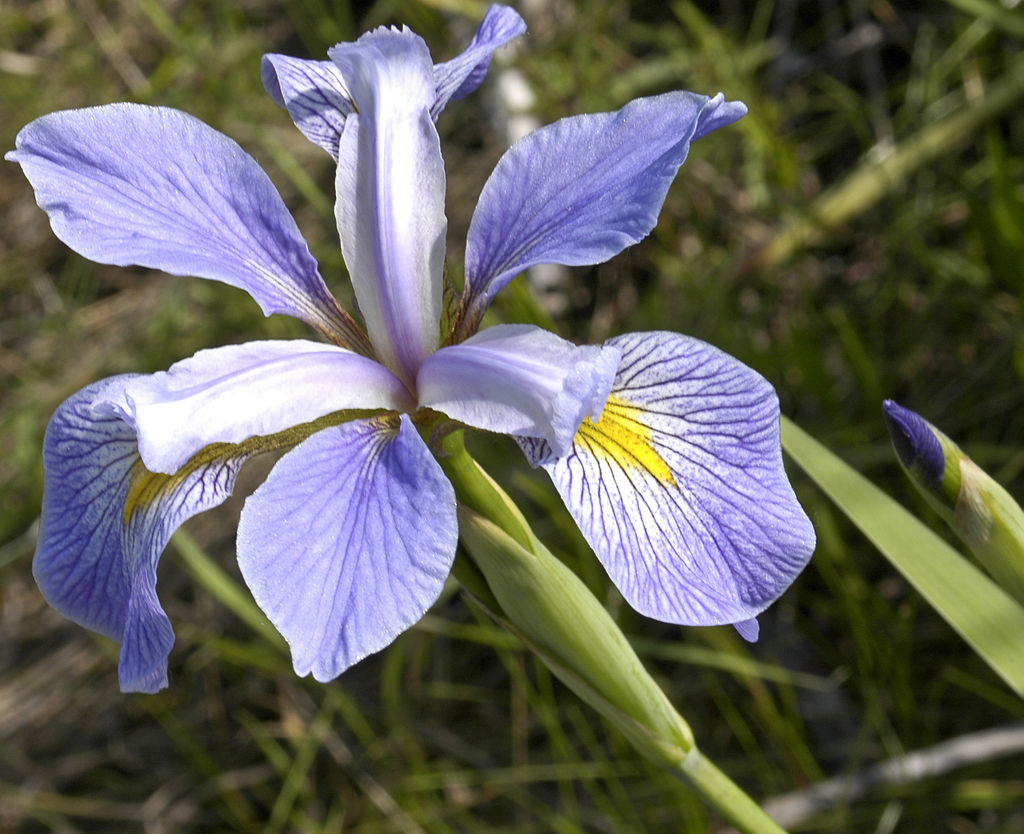
\includegraphics[width=3cm,height=3cm]{virginica}
  \caption{$\textit{Virginica}$}
\endminipage
\end{figure}
\end{frame}
%%%%%%%%%%%%%%%%%%%%%%%%%%%%%%%%%%%%%%%%%%%%%%%%%%%%%%%%%%%%%%%%%%%%%%%%%%%%%%%%%%%%
\begin{frame}{Write Your Rules}
\begin{center}
\textbf{Input} $\Rightarrow$ \textbf{Analysis} $\Rightarrow$ \textbf{Output}\newline
\end{center}
\textbf{Rules of Classification:}
   \begin{itemize}
   	\item Color,
   	\item Stalk,
	\item Sepal,
	\item Petal,
	\item ...

\end{itemize}
\end{frame}
%%%%%%%%%%%%%%%%%%%%%%%%%%%%%%%%%%%%%%%%%%%%%%%%%%%%%%%%%%%%%%%%%%%%%%%%%%%%%%%%%%%%
\begin{frame}{Features: Sepal (length, width) and Petal (length, width)}
    \begin{center}
	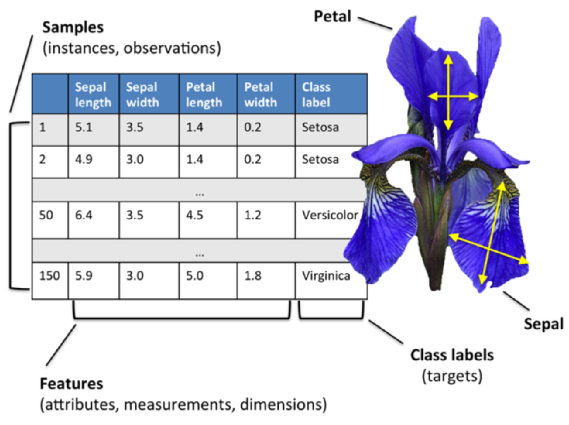
\includegraphics[height=7cm,width=11cm]{8}
	\end{center}
\end{frame}
%%%%%%%%%%%%%%%%%%%%%%%%%%%%%%%%%%%%%%%%%%%%%%%%%%%%%%%%%%%%%%%%%%%%%%%%%%%%%%%%%%%%
\begin{frame}{Classifier}
\textbf{Classifier}: is function that takes data as input and assign labels to it as output.\\
- To write classifier automatically is called supervised learning.\\
- Classifier finds the patterns in the input data.\newline \newline
\textbf{Types of classifiers:}
\begin{itemize}
\item Artificial Neural Networks;
\item Support Vector Machine;
\item Decision Tree;
\item ...
\end{itemize}
\begin{center}

\includegraphics[scale=0.4]{5}
\end{center}
\end{frame}
%%%%%%%%%%%%%%%%%%%%%%%%%%%%%%%%%%%%%%%%%%%%%%%%%%%%%%%%%%%%%%%%%%%%%%%%%%%%%%%%%%%%
\begin{frame}{Decision Tree}
\begin{center}
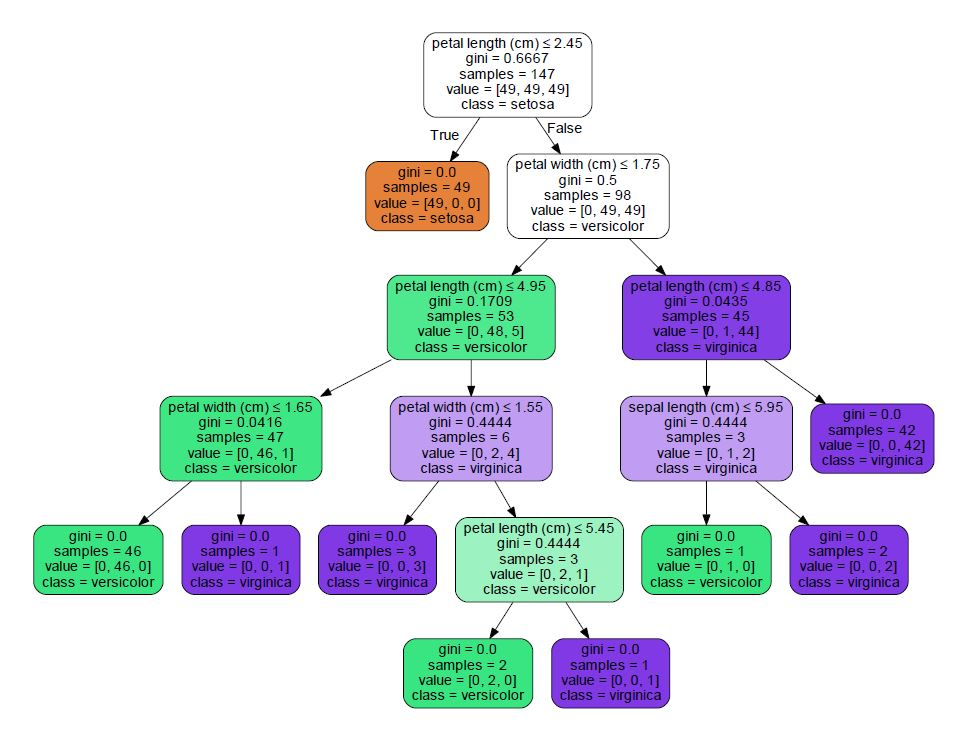
\includegraphics[scale=0.4]{tree}
\end{center}
\end{frame}
%%%%%%%%%%%%%%%%%%%%%%%%%%%%%%%%%%%%%%%%%%%%%%%%%%%%%%%%%%%%%%%%%%%%%%%%%%%%%%%%%%%%

\begin{frame}{Application}
\end{frame}
\end{document}
